\section{Introduction}
\label{sec:intro}

The model checking of higher-order recursion schemes (\emph{recursion 
schemes}, for short) has been extensively 
studied~\cite{Knapik2002,Ong2006,Kobayashi2009a}, and recently applied 
to verification of functional 
programs~\cite{Kobayashi2009,Kobayashi2009c,Kobayashi2010}. Recursion 
schemes are grammars for describing infinite 
trees~\cite{Knapik2002,Ong2006}, and the recursion scheme model checking 
is concerned about whether the tree generated by a recursion scheme 
satisfies a given property.
%% (expressed by a modal \(\mu\)-calculus formula).
It can be considered an extension of finite state and pushdown model 
checking, where the model checking of order-0 and order-1 recursion 
schemes respectively correspond to finite state and pushdown model 
checking. From a programming language point of view, a recursion scheme 
is a term of the simply-typed, call-by-name \(\lambda\)-calculus with 
recursion and tree constructors, which generates a single, possibly 
infinite tree. Various verification problems for functional programs
%%(including reachability, flow analysis, and resource usage verification~\cite{Igarashi2005})
can be easily reduced to recursion scheme model checking 
problems~\cite{Kobayashi2009,Kobayashi2009c,Kobayashi2010}. Thanks to 
the decidability of recursion scheme model checking~\cite{Ong2006}, the 
reduction yields a sound, complete, and automatic verification method 
for programs written in the simply-typed \(\lambda\)-calculus with 
recursion and \emph{finite} data domains (such as booleans).

There is, however, still a large gap between the programs handled by the 
above-mentioned method and real functional programs. One of the main 
limitations is that infinite data domains such as integers and lists 
cannot be handled by the recursion scheme model checking. To overcome 
that limitation, this paper extends the techniques of predicate 
abstraction~\cite{Graf1997} and counterexample-guided abstraction 
refinement (CEGAR)~\cite{Clarke2003a,Ball2002} for higher-order model 
checking (i.e., recursion scheme model checking).

The overall structure of our method is shown in Figure~\ref{fig:cegar}. 
Given a higher-order functional program, predicate abstraction is first 
applied to obtain a higher-order boolean program (Step 1 in 
Figure~\ref{fig:cegar}). For example, consider the following program 
\(M_1\):
\begin{verbatim}
let f x g = g(x+1) in let h y = assert(y>0) in
let k n = if n>0 then f n h else () in k(randi())
\end{verbatim}
Here, \texttt{assert} takes a boolean as an argument and is reduced to 
\texttt{fail} if the argument is false. The function \texttt{randi} 
returns a non-deterministic integer value. Using a predicate \(\lambda 
x.x>0\), we obtain the following higher-order boolean program \(e_1\):
\begin{verbatim}
let f b g = if b then g(true) else g(randb()) in
let h c = assert(c) in
let k () = if randb() then f true h else () in k()
\end{verbatim}
Here, \texttt{randb} returns a non-deterministic boolean value. Note 
that the integer variables \verb|x| and \verb|y| have been replaced by 
the boolean variable \texttt{b} and \texttt{c} respectively, which 
represents whether the values of \texttt{x} and \texttt{y} are greater 
than \(\texttt{0}\). In the abstract version of \texttt{f}, \texttt{b} 
being true means that \texttt{x>0}, which implies \texttt{x+1>0}, so 
that \texttt{true} is passed to \texttt{g} in the then-part. In the 
else-part, \(\texttt{x<=0}\), hence \(\texttt{x+1>0}\) may or may not 
hold, so that a non-deterministic boolean value is passed to \texttt{g}. 
The higher-order boolean program thus obtained is an abstraction of the 
source program; for any reduction sequence of the source program, there 
is a corresponding reduction sequence of the higher-order boolean 
program (but not vice versa). Thus, for example, if the abstract program 
does not cause an assertion failure, neither does the source program.

The higher-order boolean program is then represented as a recursion 
scheme and model-checked by using an existing recursion scheme model 
checker~\cite{Kobayashi2009,Kobayashi2009d} (Step~2 in 
Figure~\ref{fig:cegar}). 
%
If the higher-order boolean program satisfies a given safety 
property,\footnote{For the sake of simplicity, throughout the paper, we 
only consider the reachability property.} the source program is also 
safe. Otherwise, an error path of the boolean program is inspected 
(Step~3 in Figure~\ref{fig:cegar}). If it is also an error path of the 
source program, then it is reported that the program is unsafe. 
Otherwise, new predicates are extracted from the error path, in order to 
refine predicate abstraction (Step~4 in Figure~\ref{fig:cegar}).

In the example above, we actually start predicate abstraction with the 
empty set of predicates, and obtain the following abstract program 
\(e_0\):
\begin{verbatim}
let f g = g() in let h () = assert(randb()) in
let k () = if randb() then f h else () in k()
\end{verbatim}
The model checking of this program yields the following reduction 
sequence, leading to an assertion failure:
\[
\begin{array}{l}
\texttt{k()}
\red 
\texttt{if randb() then f h else ()}\\
\red 
\texttt{if true then f h else ()}
\red \texttt{f h}\\
\red \texttt{h()} \red \ASSERT(\texttt{randb()})\\
\red
\ASSERT(\texttt{false}) \red \FAIL
\qquad \qquad \qquad {\cdots(1)}
\end{array}
\]
The corresponding reduction sequence in the source program \(M_1\) is:
\[
\begin{array}{l}
\texttt{k}\, \texttt{n} \red \texttt{if n>0 then f n h else ()}\red_{\texttt{n>0}} \texttt{f n h} \\
\red \texttt{h(n+1)} \red \ASSERT{\texttt{(n+1>0)}} \red_{\texttt{n+1<=0}} \FAIL
\quad {\cdots(2)}
\end{array}
\]
Here, \(\texttt{n}\) is some integer, and we have annotated the sequence 
with the conditions that should hold at each step. As \(\texttt{n>0} 
\land \texttt{n+1<=0}\) is unsatisfiable, we know that the reduction 
sequence above is actually infeasible, so that the source program may 
not cause an assertion failure. From the unsatisfiable constraint above, 
we can learn that information about whether an integer is positive is 
useful. By using it, we get the refined abstract program shown earlier. 
As the new abstract program is safe (i.e. does not cause an assertion 
failure), we can conclude that the source program is also safe.

The idea sketched above is basically the same as the techniques for 
predicate abstraction and CEGAR used already in finite state and 
pushdown model checking~\cite{Clarke2003a,Ball2002}, except that models 
have been replaced by higher-order boolean programs (or recursion 
schemes). 
%%The idea is natural and unsurprising; Indeed, 
%%We have already suggested such an approach in our previous paper~\cite{Kobayashi2009}
%%(but without formally defining or implementing it), but
As discussed below, however, it turned out that there are many 
challenging problems in developing effective methods for predicate 
abstraction and CEGAR for higher-order model checking.

\begin{figure}
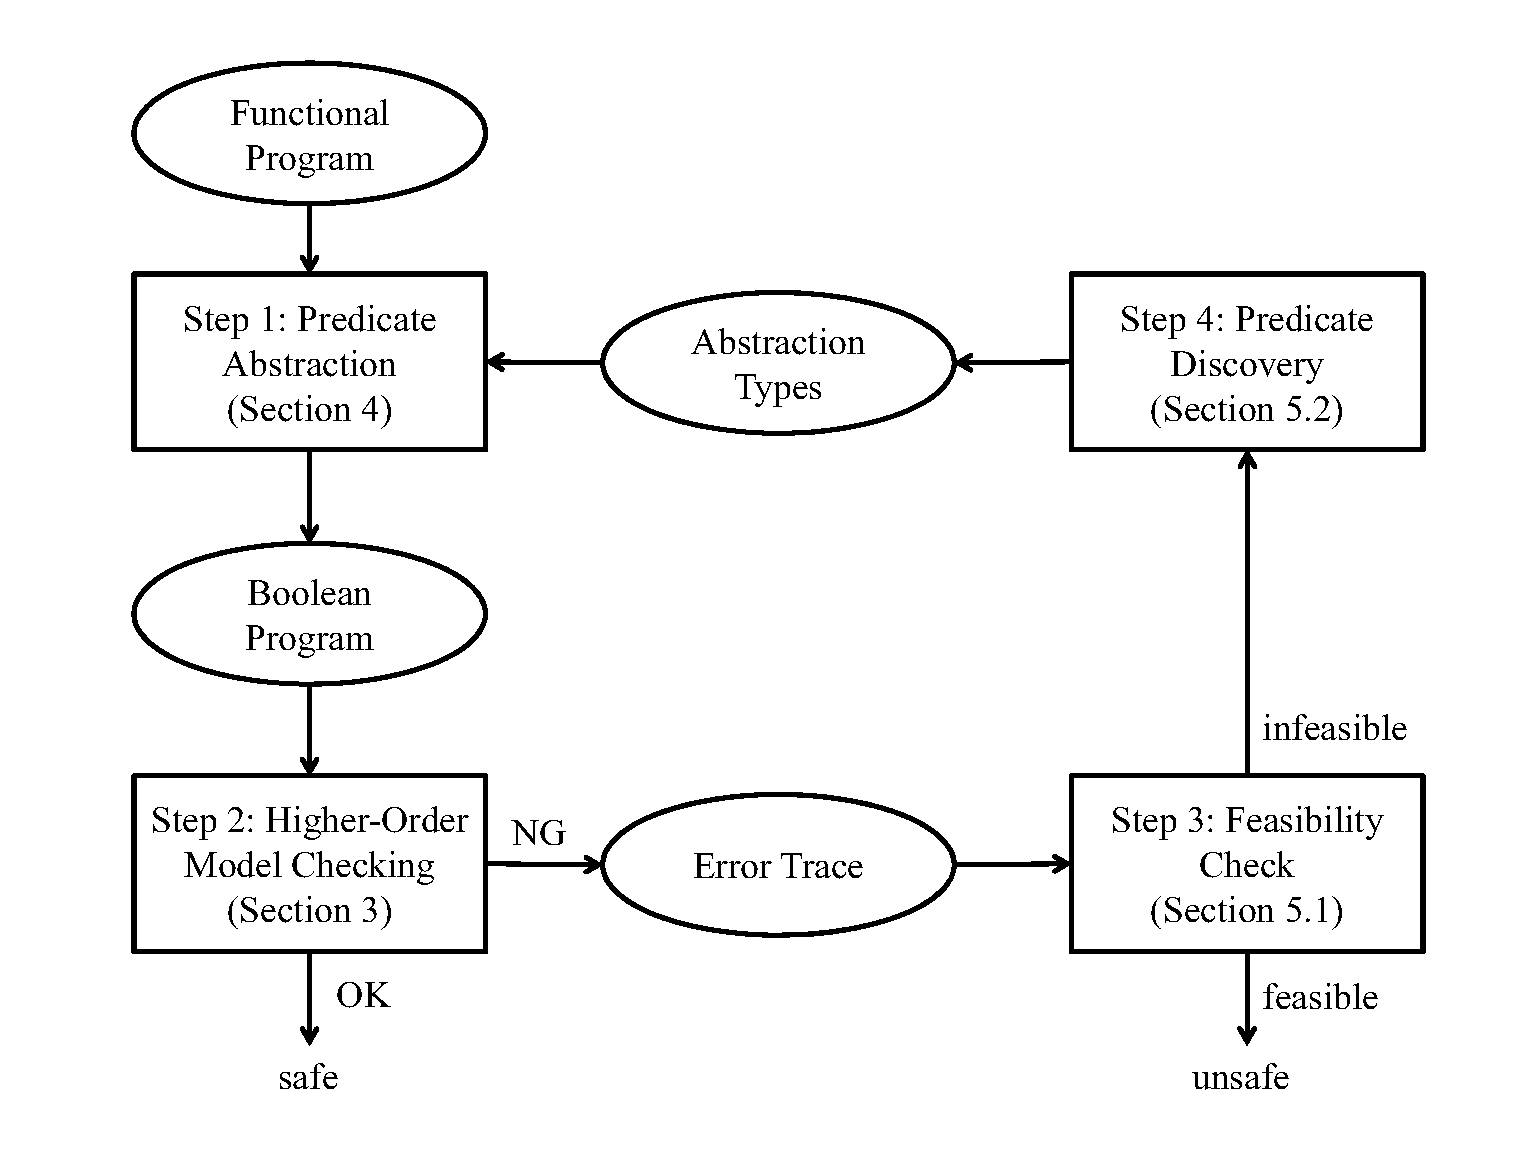
\includegraphics[scale=0.35]{overall.eps}
\caption{Higher-Order Model Checking with Predicate Abstraction and CEGAR}
\label{fig:cegar}
\end{figure}

First, for predicate abstraction, it is unreasonable to use the same set 
of predicates for all the integer variables. For example, let us modify 
the program above into the following program \(M_2\):
\begin{verbatim}
let f x g = g(x+1) in let h y = assert(y>0) in
let k n = if n>=0 then f n h else () in k(randi())
\end{verbatim}
Then, the predicate \(\lambda \nu.\nu\geq 0\) should be used for 
\texttt{x}, while \(\lambda \nu.\nu>0\) should be used for \texttt{y}. 
We should consistently use predicates; for example, with the choice of 
the predicates above, \verb|g|'s argument should be abstracted by using 
\(\lambda \nu.\nu>0\), rather than \(\lambda \nu.\nu\geq 0\). We use 
\emph{types} (called \emph{abstraction types}) to express which 
predicate should be used for each variable. For example, for the above 
program, the following abstraction types are assigned to \(f\), \(h\), 
and \(k\):
\[
\begin{array}{l}
f\COL \ITint{\lambda \nu.\nu\geq 0} \ra (\ITint{\lambda \nu.\nu> 0} \ra \TUNIT) \ra \TUNIT\\
h \COL \ITint{\lambda \nu.\nu> 0} \ra \TUNIT\qquad
%%k\COL \ITint{\lambda \nu.\nu>0}\ra\TUNIT
k\COL \ITint{\,}\ra\TUNIT
\end{array}
\]
The type of \(f\) means that the first argument of \(f\) should be an 
integer abstracted by the predicate \(\lambda \nu.\nu\geq 0\), and the 
second argument be a function that takes an integer abstracted by the 
predicate \(\lambda \nu.\nu>0\) as an argument and returns a unit 
value.\footnote{Here, abstraction types should not be confused with 
refinement types~\cite{Xi1999}; the abstraction type of a term only 
tells how the term should be abstracted, not what are possible values of 
the term. For example, integer \(3\) can have type \(\INT[\lambda 
\nu.\nu<0]\) (and it will be abstracted to the boolean value 
\textit{false}).} By using these abstraction types, the problem of 
checking that predicates are consistently used boils down to a type 
checking problem. For example, the standard rule for application:
\[
\frac{\Gamma \p M: \tau_1 \ra \tau_2\andalso \Gamma\p N:\tau_1}
{\Gamma\p M N: \tau_2}
\]
%%\infrule{\Gamma \p M: \tau_1 \ra \tau_2\andalso \Gamma\p N:\tau_1}
%%  {\Gamma\p M N: \tau_2}
ensures that \(N\) is abstracted using the predicates expected by the 
function \(M\); there is no such case that an abstraction of function 
\(M\) expects a value abstracted by using the predicate \(\lambda 
\nu.\nu>0\) but the actual argument \(N\) is abstracted by using 
\(\lambda \nu.\nu\geq0\).

A further twist is necessary to deal with multi-ary predicates.
For example, consider the following modified version \(M_3\):
\begin{verbatim}
let f x g = g(x+1) in let h z y = assert(y>z) in
let k n = if n>=0 then f n (h n) else () in
   k(randi())
\end{verbatim}
The variable \texttt{y} should now be abstracted by using %%the predicate 
\(\lambda \nu.\nu>\texttt{z}\), which 
depends on the value of \texttt{z}. Thus, %%the abstraction types introduced above should be \emph{dependent} types.
the above program should be abstracted by using the following \emph{dependent} abstraction types:
\[
\begin{array}{l}
f\COL (x\COL\ITint{\,} \ra (w\COL\ITint{\lambda \nu.\nu> x} \ra \TUNIT) \ra \TUNIT) \\
h\COL (z\COL\ITint{\,} \ra y\COL\ITint{\lambda \nu.\nu> z} \ra \TUNIT)\qquad
k\COL \ITint{\,}\ra\TUNIT
\end{array}
\]
Here, please note that the types of the second arguments of \(f\) and 
\(h\) refer to the values of the first arguments. Thus, our type system 
for ensuring the consistency of predicates is actually a \emph{dependent} 
one. A predicate abstraction algorithm is then formalized as a 
type-directed transformation relation \(\Gamma \p M:\tau \Rightarrow e\) 
based on the dependent abstraction type system, where \(M\) is a source 
program and \(e\) is an abstract program.\footnote{To avoid the 
confusion, we call dependent abstraction types just \emph{abstraction 
types} below. We use the term ``dependent types'' to refer to ordinary 
dependent types 
%%(such as
%%\(x\COL\rtbase{\nu}{\INT}{\nu>0}\ra \rtbase{\nu}{\INT}{\nu>x}\), which describe functions that
%%a positive integer \(x\) as input and returns an integer greater than \(x\))
used for expressing refinement of simple types.}

%\koba{Below, we should be careful about what we mean by ``dependent type system''.
%Should we instead use the word ``refinement type system''?}
%
The predicate abstraction mentioned above is sound in the sense that if 
an abstract program is safe (i.e., does not reach \texttt{fail}), so is 
the source program. Further, we can show that it is relatively complete 
with respect to a dependent (refinement) intersection type 
system~\cite{Terauchi2010}: If a source program is typable in the 
dependent intersection type system, our predicate abstraction can 
generate a safe abstract boolean program by using certain abstraction 
types.
%% containing the atomic predicates occurring in the dependent intersection types.
This means that, as long as suitable predicates are provided (by a user 
or an automated method like the CEGAR discussed below), the combination 
of our predicate abstraction and higher-order model checking has at 
least the same verification power as (and actually strictly more 
expressive than, as discussed later: see 
Remark~\ref{rem:more-expressive-than-deptype} in Section~\ref{sec:pred}) 
the dependent intersection type system. Here, note that we need only 
atomic predicates used in the dependent types; higher-order model 
checking can look for arbitrary boolean combinations of the atomic 
predicates as candidates of dependent types. Thus, this part alone 
provides a good alternative to Liquid types~\cite{Rondon2008}, which 
also asks users to provide templates of predicates, and infers dependent 
types. Thanks to the power of higher-order model checking, however, our 
technique can infer dependent, \emph{intersection} types unlike Liquid 
types.
%(This point is discussed in more detail later. )


We now discuss the CEGAR part. Given an error path of an abstract 
boolean program, we can find a corresponding (possibly infeasible) error 
path of the source program. Whether the error path is feasible in the 
source program can be easily decided by symbolically executing the 
source program along the error path, and checking whether all the 
branching conditions in the path are satisfiable (recall the example 
given earlier). The main question is, if the error path turns out to be 
infeasible, how to find a suitable refinement of abstraction types, so 
that the new abstraction types yield an abstract boolean program that 
does not contain the infeasible error path. This has been well studied 
for first-order 
programs~\cite{Ball2001,Ball2002,Ball2005,Heizmann2010,Clarke2003a,Henzinger2002,Henzinger2004},
%
but it is not clear how to lift those techniques to deal with 
higher-order programs.

Our approach to finding suitable abstraction types is as follows.
%%dependent type inference~\cite{Terauchi2010}.
From a source program and its infeasible error path, we first construct 
a \emph{straightline higher-order program} (abbreviated to SHP) that 
exactly corresponds to the infeasible path, and contains neither 
recursion nor conditional branches. In the case of the program \(M_3\) 
above, this is easily obtained, as follows:
\begin{verbatim}
let f1 x g = g(x+1) in let h1 z y = assert(y>z) in
let k1 n = assume(n>=0); f1 n (h1 n) in k1(c)
\end{verbatim}
Here, \texttt{c} is a constant, and \(\texttt{assume}(b)\) evaluates 
\(b\), and proceeds to the next instruction only if \(b\) is true. (But 
unlike \texttt{assert}, it is not reduced to \texttt{fail} even if \(b\) 
is false.) For general programs that contain recursions, the 
construction is more involved: see Section~\ref{sec:cegar}.
%%as shown in Section~\ref{sec:cegar}, a function in the source program
%%may need to be duplicated (i.e., for each function \(f\) in the source program,
%%there may be more than one corresponding function \(f_1,\ldots,f_k\)).

For SHP, a standard dependent (refinement) type system is sound and 
\emph{complete}, in the sense that a program does not reach \texttt{fail} 
if and only if the program is typable in the type system. Further, (a 
sub-procedure of) previous algorithms for inferring dependent types 
based on interpolants~\cite{Unno2009,Terauchi2010} is actually complete 
(modulo the assumption that the underlying logic is decidable and 
interpolants can always be computed) for SHP. Thus, we can automatically 
infer the dependent type of each function in the straightline program. 
For example, for the program above, we obtain:
\[
\begin{array}{l}
\texttt{f1}: (\rtfunb{x}{\INT}
{\rtfun{(\rtfunb{y}{\rtbase{\nu}{\INT}{\nu>x}}{\TUNIT})}{\TUNIT}}) \\
\texttt{h1}: (\rtfunb{z}{\INT}
        {\rtfunb{y}{\rtbase{\nu}{\INT}{\nu>z}}{\TUNIT}}) \\
\texttt{k1}: (\rtfunb{z}{\INT}{\TUNIT})
\end{array}
\]
Here, the type of \texttt{h1} means that given integers \(z\) and \(y\) 
such that \(y>z\), \(\texttt{h1}\,z\,y\) returns a unit value without 
reaching \texttt{fail}. (These dependent types should not be confused 
with abstraction types: the latter only provides information about how 
the source program should be abstracted.)

We then refine the abstraction type of each function in the source 
program with predicates occurring in the dependent types of the 
corresponding functions in the SHP. For example, given the above 
dependent types, we get the following abstraction types:
%%for the source program:
\[
\begin{array}{l}
\texttt{f}: (x\COL\TINT[\,]\ra (y\COL\TINT[\lambda \nu.\nu>x]\ra \TUNIT)\ra\TUNIT) \\
\texttt{h}: (z\COL\TINT[\,]\ra y\COL \TINT[\lambda \nu.\nu>z]\ra \TUNIT) \qquad
\texttt{k}: \ITint{\,}\ra\TUNIT
\end{array}
\]
We can show that the abstraction types inferred in this manner are 
precise enough, in that the abstract program obtained by using the new 
abstraction types no longer has the infeasible error path. (Thus, the 
so-called ``progress'' property is guaranteed as in CEGAR methods for 
finite-state or pushdown model checking.)

%%%From a source program and a spurious 
%%%For first-order programs, 
%%%\koba{Rewrite the paragraph below, to reflect the new CEGAR method.
%%%Also, mention somewhere in the introduction about the properties satisfied by predicate abstraction
%%%and cegar.}
%%%From the simple types of a source program, one can first obtain a ``template'' of
%%%abstraction types. For example, for the last program above, we obtain:
%%%\[
%%%\begin{array}{l}
%%%\hspace*{-.5cm}f\COL (x\COL\ITint{\lambda x.\seq{P_1}(x)}) \ra (w\COL\ITint{\lambda y.\seq{Q_1}(x,y)} \ra \TUNIT) \ra \TUNIT\\
%%%h \COL (z\COL\ITint{\lambda x.\seq{P_2}(x)}) \ra (y\COL\ITint{\lambda y.\seq{Q_2}(z,y)}) \ra \TUNIT\\
%%%n\COL \ITint{\lambda n.\seq{P_3}(n)}
%%%\end{array}
%%%\]
%%%Here, \(\lambda x.\seq{P_i}(x)\) represents a sequence of predicates 
%%%\(\lambda x.P_{i1}(x)\), \(\ldots,\lambda x.P_{ik}(x)\).
%%%The goal of CEGAR is to find, from a counterexample, predicates that should occur 
%%%in the sequences of predicates above.
%%%For that purpose, we can use an interpolating theorem prover, following the interpolant-based technique
%%%for CEGAR in finite state model checking~\cite{Henzinger2004}.
%%%For formulas \(P\) and \(Q\) such that \(P\land Q\) is unsatisfiable,
%%% a \emph{Craig interpolant} of \(P\) and \(Q\) is a formula
%%%\(R\) such that \(P\IMPLY R\) and \(R\IMPLY \neg Q\), with \(\FV{R}\subseteq \FV{P}\cap \FV{Q}\).
%%%Intuitively, \(R\) is a simple justification of why \(P\land Q\) is unsatisfiable. For example,
%%%\(R \equiv x>0\) is an interpolant of \(P \equiv x+y>0 \land y<0\) and 
%%%\(Q \equiv x+z<0 \land z=1\); it is a \emph{simple} justification
%%% in the sense that it refers to only the variables common between the two formulas.
%%%
%%%To see how interpolants can be used in CEGAR, let us consider 
%%% the first program \(M_1\) and the infeasible error path (2).
%%%From the infeasible error path, we get the following sequence of constraints, each of which corresponds to 
%%%a branch condition or a variable binding.
%%%\[
%%%n>0; x=n; y=x+1; \neg(y>0)
%%%\]
%%%Let us cut the above sequence of constraints into \(C_1=\set{n>0,x=n,y=x+1}\) and \(C_2=\set{\neg(y>0)}\).
%%%Note that \(C_1\land C_2\) is unsatisfiable. %%, in other words, \(\forall x,y,n.(\land C_1 \implies \neg (\land C_2))\) holds.
%%%By using an interpolating theorem prover~\cite{Beyer2008,McMillan2005}, one can obtain \(y>0\) as an interpolant of \(\land C_1\) and 
%%%\(\land C_2\). We can use this as a predicate for abstracting \(y\). 
%%%By cutting the sequence of constraints above in other positions, one can also get \(n>0\) and \(x>0\) as interpolants.
%%%Thus, we can use these predicates to abstract the first program.
%%%This idea is basically the same as the interpolant-based CEGAR for imperative programs~\cite{Henzinger2004}.
%%%
%%%A further twist is, however, required for finding predicates in higher-order model checking.
%%%Recall the program \(M_3\). Using the coarsest abstraction, we get the following false error path:
%%%\[
%%%\begin{array}{l}
%%%\texttt{if n>0 then f n (h n) else ()}\red_{n>0} \texttt{f n (h n)}\\
%%%\red \texttt{h n (n+1)} \red \ASSERT{\texttt{(n+1>n)}} \red_{\neg(n+1>n)} \FAIL \\
%%%\hfill\qquad {\cdots(3)}
%%%\end{array}
%%%\]
%%%The corresponding sequence of constraints, representing branch conditions and variable bindings, is:
%%%\[
%%%n>0;\, x=n;\, g=h\, n;\, z=n;\, y=n+1;\, \neg(n+1>n).
%%%\]
%%%From this sequence, however, it is not clear how to extract predicates
%%%that should be used in the template of abstraction type of \(f\):
%%%\[
%%%(x\COL\ITint{\lambda x.\seq{P_1}(x)}) \ra (w\COL\ITint{\lambda w.\seq{Q_1}(x,w)} \ra \TUNIT) \ra \TUNIT
%%%\]
%%%First, the above constraints contain an equality \(g=h\,n\) on functions.
%%%Second, we need to find binary predicates \(\seq{Q_1}(x,w)\) that co-relate \(x\) and \(w\), but
%%%\(w\) does not occur in the sequence above.
%%%In Section~\ref{sec:cegar}, we show (i) how to systematically generate, from an infeasible error path,
%%%constraints (on first-order variables, not on function variables)
%%% that contain information about the co-relations on variables needed in the template of abstraction types,
%%%and (ii) how to re-arrange the constraints so that interpolating theorem provers can be used
%%%to find suitable predicates.
%%%
%%%As mentioned above, our techniques of predicate abstraction and CEGAR for higher-order model checking
%%%are non-trivial extensions of those for finite state or pushdown model checking.

Based on the predicate abstraction and CEGAR techniques mentioned above, 
we have implemented a prototype verifier for (simply-typed) higher-order 
functional programs with recursion and integer base types, and tested it 
for several programs.

Our contributions include: (i) the formalization of predicate 
abstraction for higher-order programs, based on the novel notion of 
abstraction types, (ii) the formalization of CEGAR for higher-order 
programs, based on the novel notion of SHP and reduction of the 
predicate discovery problem to dependent type inference, (iii) 
theoretical properties like the relative completeness of our method with 
respect to a dependent intersection type, the progress property, etc., 
and (iv) the implementation and preliminary experiments.
%%that shows the feasibility of our method (at least for small programs).
%%, despite the extremely high worst-case complexity of higher-order model checking.

The rest of this paper is structured as follows. Section~\ref{sec:lang} 
introduces the source language, and Section~\ref{sec:boolean} introduces 
a language of higher-order boolean programs, and reviews the result on 
higher-order model checking.
%%a higher-order functional programming language with recursion and integer base types
%%as the target of our verification framework.
%%Section~\ref{sec:boolean} introduces a language of higher-order boolean programs, and reviews the result
%%on higher-order model checking (restated for higher-order boolean programs, instead of recursion schemes).
Sections~\ref{sec:pred} and \ref{sec:cegar} respectively formalize 
predicate abstraction and CEGAR for higher-order programs. 
Section~\ref{sec:experiment} reports our prototype implementation and 
preliminary experiments. Section~\ref{sec:related} discusses related 
work, and Section~\ref{sec:conc} concludes.
\iffull
\else
For the space restriction, proofs are omitted, which are available in a 
full version~\cite{Kobayashi2011}.
\fi

%%%In this paper, we propose a verification method ..
%%%
%%%The overall structure of our method is shown in ...
%%%%
%%%For ..., we use a technique called predicate abstraction, which is originally proposed by \cite{Graf1997}.
%%%Translate a program that manipulates infinite data domains 
%%%into a Boolean program whose event sequences over-approximate those of 
%%%the original program.
%%%predicate abstraction for first-order programs is proposed by \cite{Ball2005}.
%%%We investigate predicate abstraction for higher-order programs.
%%%%
%%%For higher-order programs, we have two challenges. The first challenge 
%%%is how to specify predicates. problem: variable scope. Solution: To deal 
%%%with the problem, we use a kind of dependent types to specify predicates. 
%%%The second challenge is how to make abstraction of higher-order programs. 
%%%Problem1: relating the actual and formal argumnets and the return value 
%%%for abstracting higher-order function calls. Solution: type-directed 
%%%translation. especially, type coercions. problem2: cost for computing 
%%%best possible abstraction. solution: ???.
%%%
%%%%
%%%The counterexample-guided abstraction refinement (CEGAR).
%%%Problem: variable scope?? solution: constraint partitioning?
%%%
%%%We overview our method by using the following example: \todo{use a 
%%%practical, higher-order, and simple example}
%%%%
%%%\todo{summation of f(0), ..., f(n)?}
%%%
%%%The rest of the paper is organized as follows. ...
